\section{Results}
We now describe the results of our comparison between the HIGHLIGHTS strategy summarization method and our novel \disalg~ approach. We report the main experimental results with respect to the hypotheses raised in the previous section. 

Figure \ref{fig: DA HL compare} shows the percentage of participants who were successful in answering the experiment tasks in each of the experiment conditions, for each agent pair combination.

\emph{(H1) Participants in the HIGHLIGHTS condition struggled to successfully identify the better
performing agent in the comparison task.} When all agents are of decent performance, we see the difficulty
of distinguishing between them manifest itself in a poor success rate.
Based on participants' textual explanations of the choice of agent, it seems they were concerned that agent $E$ was indecisive, e.g., ``[Agent $E$] seems very indecisive while ... [Agent $M$] seems to have a plan and is going with it.''. %,  ``... [Agent $E$] behaved more like a human.''
We hypothesize that these responses are a consequence of a single trajectory in agent $E$'s summary where the frog is seen leaping between logs in a seemingly indecisive manner. These results emphasize the limitations of independent comparisons.
% summaries and strengthen our claims regarding their limitations.
% \ya{changed, but didn't mention anything regarding a random guess, not sure it's necessary}

% A Bootstrap analysis shows that in such a case,
% selecting the better performing agent is \emph{not} significantly different from a random guess  ($p > 0.59$ for all agent pairs).

% with  $(p =
% 0.59)$ for $E$ vs. $LV$, $(p = 0.595)$ for $E$ vs. $M$ and $(p = 0.595)$ for $LV$ vs. $M$. 

\emph{(H2) Participants in the \disalg~ condition were more successful in the agent comparison
task}. Participants in the \disalg~ group 
% given the same agents to compare, 
showed vast improvement
in the ability to identify the better performing Frogger agent  (see Figure \ref{fig: DA HL compare}). The differences in success rate between conditions  were statistically significant and  
substantial for all agent comparisons ($E$ vs. $LV$: $p = 1.6^{-5}$; $E$ vs. $M$: $p = 1.7^{-5}$; $LV$ vs. $M$: $p = 0.018$). Textual explanations provide insights regarding how the
contrastive nature of the \disalg~ summaries helped participants decide which agent to choose, e.g. `` I preferred the path that ... [Agent $E$] was taking''; ``I felt that ... [Agent $E$] was making slightly stronger moves, and pushing ahead further''.



% Figure \ref{fig: DA HL compare} reports the comparison in the percentage of participants that were
% able to correctly identify the better performing agent between the HIGHLIGHTS and \disalg~ summary
% methods. Participants observing the HIGHLIGHTS summaries showed poor success results for comparing
% between agents $E$ and $LV$, strengthening our H1 hypothesis -- \emph{Participants shown
% HIGHLIGHTS summaries of low-varying performance agents were not always able to correctly select
% the most skilled agent.} Participant in the \disalg~ group, given the same agents to compare,
% showed vast improvement in the ability to identify the better agent, strengthening our H2
% hypothesis -- \emph{Participants shown Disagreement summaries of low-varying performance agents
% were able to correctly select the most skilled agent.} The analysis shows a statistically
% significant and substantial difference in performance when comparing \disalg~ to HIGHLIGHTS with
% $(p < 1.4^{-5})$ for $E$ vs. $LV$ and $(p < 0.15)$ for $E$ vs. $HV$.

% \ya{maybe add some of the user study comments} \oa{yes, it would be nice if you could show an
% example comment or two from DA participants that shows the direct comparison helped them}


% \begin{itemize}
% 	\item \textbf{`` I preferred the path that ... was taking''} 
% 	\item \textbf{`` I felt that ... was making slightly stronger moves, and pushing ahead
% 	further''} 
% 	\item \textbf{``Agent ... was clearly making better choices''}
% \end{itemize}
%%%other options:
% ``Agent two made better choices overall in both videos''
% ``Agent 2 made smarter moves as a whole''
% ``Agent one got himself dead in the second video, the choice is easy.''
% ``Agent..reached lily pad first... further ahead first..''



% The analysis shows statistically significant and substantial differences in performance when
% comparing user success percentage using \disalg~ compared to HIGHLIGHTS. \ref{fig: DA HL compare}


% \emph{(H1) Participants shown HIGHLIGHTS summaries of low-varying performance agents were not
% always able to correctly select the most skilled agent.}  Participants’ selection for this agent
% comparison task are shown in Figure \ref{fig: HL vote}. These results support H1. The graphs
% indicate an agreement between our study participants that agent $LV$ dominates agent $E$ which we
% know to be false. A likely cause of this outcome can simply be the different states each agent
% determines as important, which results in different summary trajectories shown. This strengthens
% our claims regarding the limitations of HIGHLIGHTS summaries for comparison tasks due to
% non-dependency between the agents. 


% \begin{figure}[ht] \centering 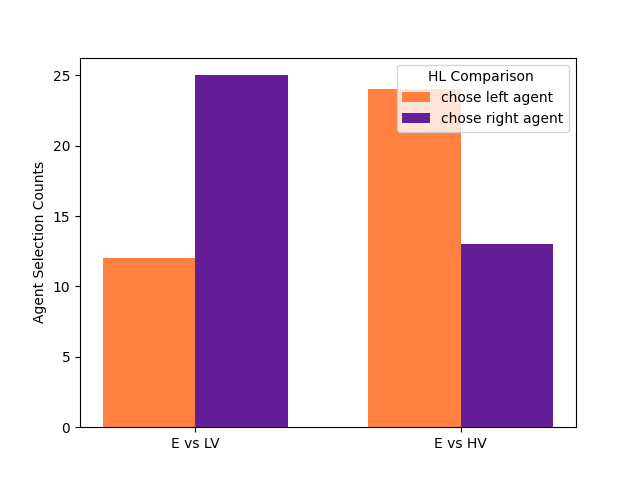
\includegraphics[width=0.75\columnwidth]{images/HL_hard_vote.png}\\
%   \vspace{-0.7cm} \caption{Agent selection using HIGHLIGHTS with low-varying performance agents}
%   \label{fig: HL vote} \vspace{-0.2cm} \end{figure}


% \emph{(H2) Participants shown Disagreement summaries of low-varying performance agents were able
% to correctly select the most skilled agent.}  Participants’ selection for this agent comparison
% task are shown in Figure \ref{fig: DA HL compare}. These results support H2. Given the same agents
% to compare, we can see a vast improvement in the user's ability to identify the better agent. 




% \begin{figure}[ht] \centering 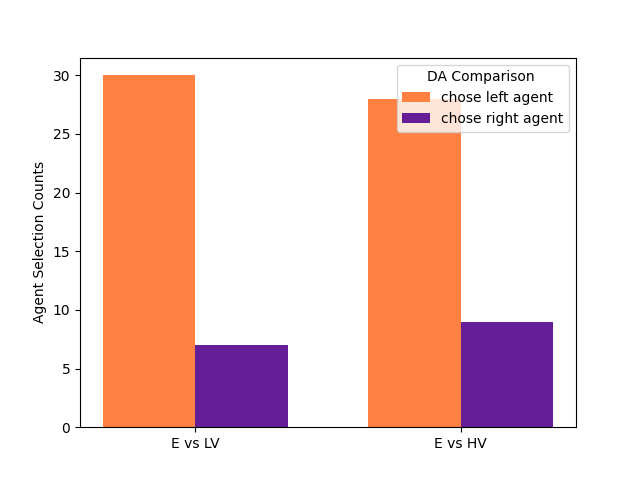
\includegraphics[width=0.75\columnwidth]{images/DA_vote.png}\\
%   \vspace{-0.7cm} \caption{Agent selection using the \disalg~ algorithm on low-varying
%   performance} \label{fig: DA vote} \vspace{-0.2cm} \end{figure}

% \begin{figure}[ht]
% 	\centering
% 	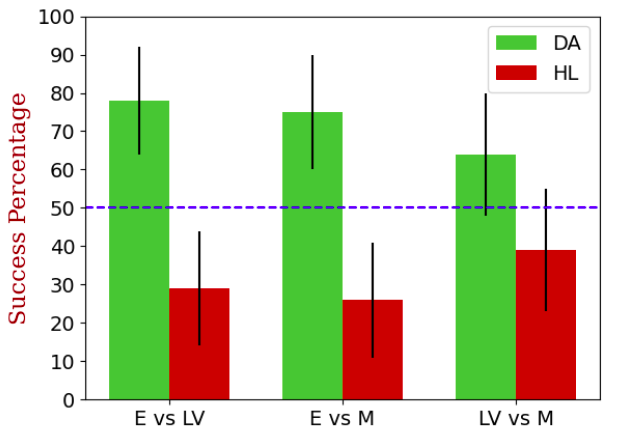
\includegraphics[width=0.75\columnwidth]{images/success.png}\\
% 	% \vspace{-0.7cm}
% 	\caption{Agent selection success percentage}
% 	\label{fig: DA HL compare}
% % 	\vspace{-0.2cm}
% \end{figure}

\emph{(H3) A significant difference was found between success rates of participants in the conveying differences task}. Participants achieved a significantly higher success rate with the \disalg~ method in the $FR$ vs. $SD$ comparison ($p = 0.014$). Albeit, this was mostly a result of the low performance of HIGHLIGHTS in $Q1$ due to the $SD$ summary containing, coincidentally, only trajectories of the agent at the bottom lane. 
The inferior performance of \disalg~ in $Q1$ of $CL$ vs. $FR$  ($p = 0.187$) can be explained by summary trajectories where no vehicles were present in $CL$'s lane allowing it to drive faster than $FR$ and appear less considerate of keeping distance.
While not necessarily outperforming it, the \disalg~ is at least equivalently useful as HIGHLIGHTS, which was shown to be better than random~\cite{Tobias}.


% \emph{(H3) Explanation satisfaction of participants shown \disalg~ summaries was similar to that of
% participants shown HIGHLIGHTS summaries.} Participants’ distributions of scores for the explanation
% satisfaction were not statistically significant $(p_{exp\#1} = 0.17, p_{exp\#2} = 0.61)$.

\emph{(H4) No clear participant preference towards one summary method was observed.} Most participants answered that both methods were equally beneficial. However,
more participants found \disalg~ more \emph{helpful} and containing less irrelevant information than HIGHLIGHTS, while finding the latter more \emph{pleasing}.



% \begin{figure}[ht]
% 	\centering
% 	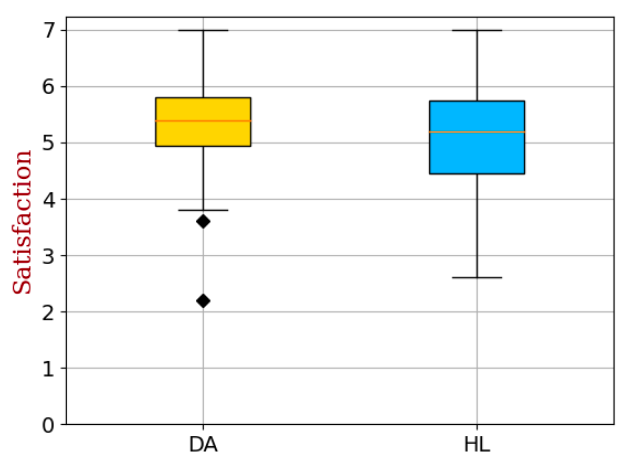
\includegraphics[width=0.65\columnwidth]{images/sat.png}\\
% % 	\vspace{-0.7cm}
% 	\caption{User satisfaction of summary methods}
% 	\label{fig: sat}
% % 	\vspace{-0.2cm}
% \end{figure}

% \emph{Confidence of correct participants.}
% Figure \ref{fig: conf}  shows the confidence
% ratings of participants who made the correct choice.\footnote{We compare the confidence ratings of
% correct participants, as being confident in a wrong choice is not desirable.} Ratings were slightly higher in two of the comparisons for the \disalg~ condition, however, none of the differences were statistically significant. 
% The analysis shows $(p = 0.68)$ for $E$ vs. $LV$, $(p  = 0.08)$ for $E$ vs. $M$ and $(p = 0.15)$ for $LV$ vs. $M$. 

\emph{Confidence and satisfaction}
In both experiments no statistically significant differences were found between the confidence or satisfaction of participants in different conditions (See Appendix).



% \emph{Correct participants in the \disalg~ condition were more confident than correct participants
% in the HIGHLIGHTS condition.} In addition to the agent selection success rate metric, we measured
% participants’ confidence in their selections. Figure \ref{fig: conf}  shows the confidence ratings
% of participants who made the correct choice\footnote{We compare the confidence ratings of correct
% participants, as being confident in a wrong choice is not desirable.}, showing that correct
% participants in the \disalg~ condition were more confident than correct participants in the
% HIGHLIGHTS condition. This difference was statistically significant for two of the three agent pairs
% ($(p < 0.017)$ for $E$ vs. $LV$ and $(p < 0.005)$ for $E$ vs. $HV$). 
% and the analysis show an increase in confidence of participants exposed to the \disalg~ summaries,
% with $(p < 0.017)$ for $E$ vs. $LV$ and $(p < 0.005)$ for $E$ vs. $HV$.


% \begin{figure}[ht]
% 	\centering
% 	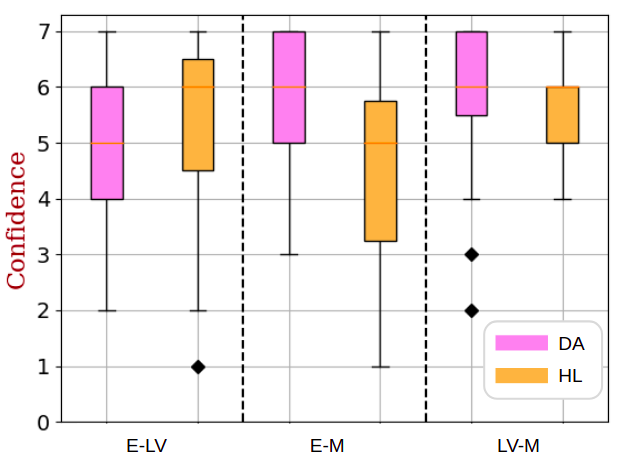
\includegraphics[width=0.65\columnwidth]{images/conf.png}\\
% 	% \vspace{-0.5cm}
% 	\caption{Confidence of correct participants}
% 	\label{fig: conf}
% % 	\vspace{-0.2cm}
% \end{figure}
